\section{Question 2}

\subsection{Question}
Download the TimeMaps for each of the target URIs.  We'll use the mementoweb.org 
Aggregator, so for example:\\

URI-R = http://www.cs.odu.edu/\\

URI-T = http://mementoweb.org/timemap/link/http://www.cs.odu.edu/\\

You could use the cs.odu.edu aggregator:\\

URI-T = http://mementoproxy.cs.odu.edu/aggr/timemap/link/1/http://www.cs.odu.edu/\\

But be sure to say which aggregator you use -- they are likely to give
different answers.\\

Create a histogram of URIs vs. number of Mementos (as computed from
the TimeMaps).  For example, 100 URIs with 0 Mementos, 300 URIs
with 1 Memento, 400 URIs with 2 Mementos, etc.\\

See: http://en.wikipedia.org/wiki/Histogram\\

Note that the TimeMaps can span multiple pages.  Look for links like:\\

<http://mementoweb.org/timemap/link/1000/http://www.cnn.com/>;rel="timemap"; 
type="application/link-format"; from ="Sun, 08 Jul 2001 21:30:54 GMT"\\

This indicates another page of the TimeMap is available.  There can be 
many pages to a TimeMap.\\

\subsection{Resources}
\begin{itemize}
\item R: \url{http://www.cs.odu.edu/~sainswor/uploads/Teaching/cs595f13-R.pdf}
\end{itemize}

\subsection{Answer}
The python script in Listing \ref{listing:memfind} was used to retrieve the timemaps and then parse the returned html, traveling down the rabbit hole if the target URI has more than 1000 mementos.

\lstinputlisting[language=Python, caption={mementofinder.py}, label=listing:memfind]{q2/mementofinder.py}

The dataset created Listing \ref{listing:memfind}. A log scale was used along the y-axis to show more detail among the results. The script in Listing \ref{listing:bld_hist} was used to create the histogram in Figure \ref{fig:hist_ss}, which shows the distribution of mementos per site from the dataset of Question 1.

\lstinputlisting[language=R, caption={build\_histogram.r}, label=listing:bld_hist]{q2/build_histogram.r}

\begin{figure}[h]
\centering
\fbox{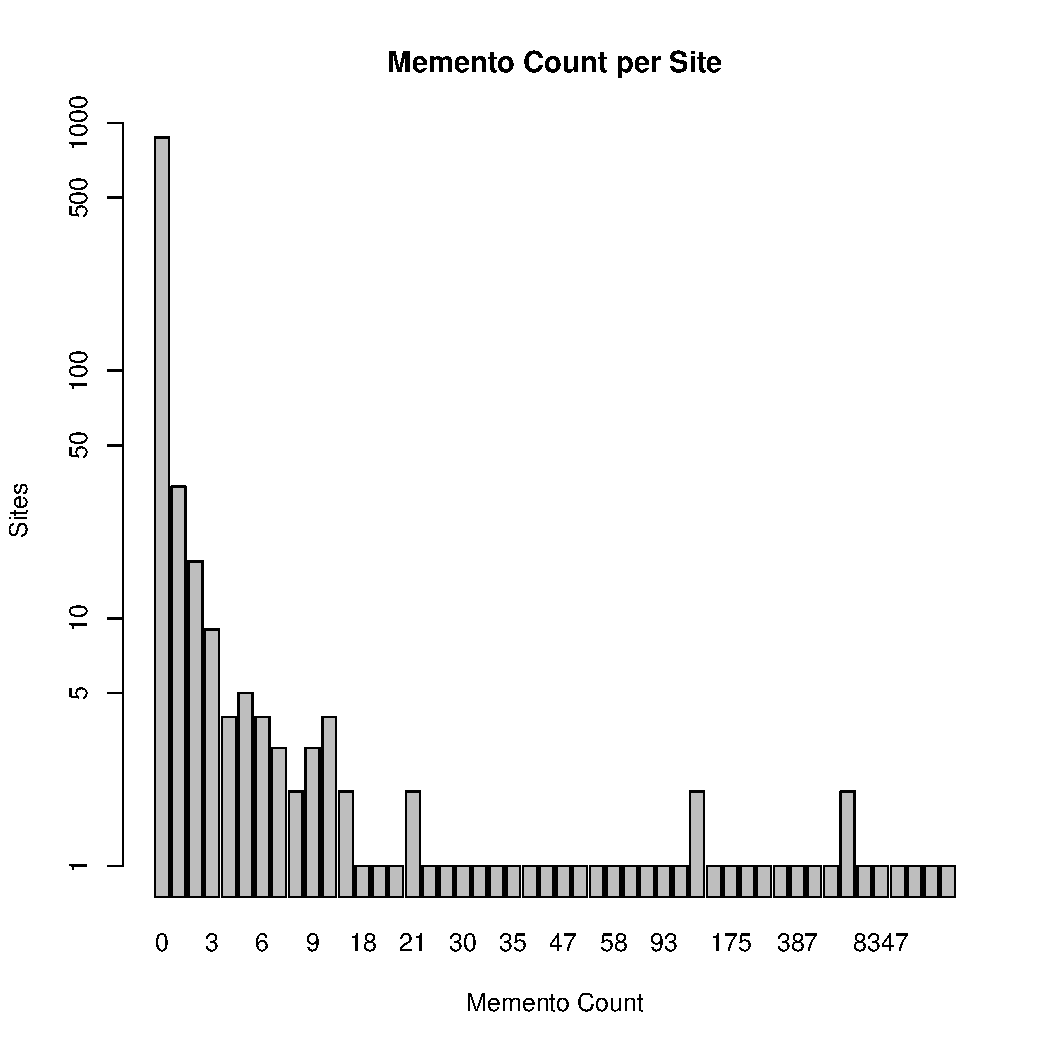
\includegraphics[scale=.65]{q2/hist.pdf}}
\caption{Histogram of Site Mementos}
\label{fig:hist_ss}
\end{figure}
